\section{Preliminary experiments}\label{sec:setup}
In this Section, we describe two preliminary experiments we conducted in Spring 2018 following the framework presented in the previous section. The first experiments is a rehearsal between two musicians in the same room, where we insert visual occlusions to test their ability to interact in adverse conditions. The second experiments is a set of rehearsals between five couples of musicians from two separate rooms, connected via a network emulator to test the sense of presence and quality of performance at different latency conditions. The results of the two experiments are discussed in the next section.


\subsection{Co-presence performance with visual occlusion}
We invited a string duo to make a pilot test of the environment, the perceptual questionnaire and the musical pieces that we intended to use for the second experiment. We also included a test on adverse conditions of the medium (visual occlusion) to qualitatively assess the importance of video feedback in NMPs.

We show a summary of the test conditions in table \ref{tab:exp1}. The two subjects are a violin and a cello player and are brothers, hence they have a long-time experience playing together and use a wide set of visual and audio cues to interact. For the musical parts, we create a composition that require mutual interaction and understanding. They include attacks, alternate scales, changes of tempo, unison playing, sustained loop. The parts are described in detail in \cite{CIM2018} and publicly available\footnote{https://tinyurl.com/intermusicCIM2018}.

The performers were asked to play in two conditions of the medium: with no visual occlusion, and with partial visual occlusion, by inserting a tulle panel between the two instrumentalists, thus providing a blurring effect on their figures (as shown in Figure \ref{fig:veli}). The aim was to observe their behavior, adaptation strategies, and emerging non-verbal communication (bodily and musical gestures).

The acquisition of the experiment was based on a subjective questionnaire on their sense of presence and free comments on the experience. 



\begin{table}
\centering
\caption{Details of the experiment in co-presence}
\begin{tabular}{p{1.5cm}p{6cm}}
\hline
\textbf{Entity} & \textbf{Properties} \\
\hline
\textbf{Performance} & Co-presence performance. \newline Parts arranged from Bartok pieces as described in [cit]. \\
\textbf{Subjects} & Two brothers, violin and cello players. \newline Violin player: male, AGE?, musical experience?; 	\newline Cello player: make, AGE?, musical experience?\\
\textbf{Environment} & Recording and mastering studio in the Conservatory of Milan; acoustically equipped with bass traps. \newline Musicians sit side by side, with peripherical vision.\\
\textbf{Medium} & Air propagation. \newline Visual occlusion applied by means of a a screen with progressive layers of canvas applied to decrease transparence and visibility. \\
\textbf{Acquisition} & Interview to the participants and free comments.\\
\hline
\end{tabular}
\label{tab:exp1}
\end{table}


\begin{figure}[t]
	\centering
	\includegraphics[width=\columnwidth]{img/veli.eps}
	\caption{The two musicians in experiment 1, with partial occlusion and blurred effect.}
	\label{fig:veli}
\end{figure}


\subsection{Sense of presence in NMPs}
Five couples of musicians, playing different combinations of instruments, took part in the experiment. Some couples never had rehearsed together, while others did. The details of the experiment are reported in Tab.~\ref{tab:exp2}

Each session of the experiment comprised a single couple, the two musicians were placed in different rooms , standing in front of a screen, in order to be connected both with respect to video and audio. An example of the setup for the couple consisting of harp and flute is shown in Fig.~\ref{fig:afsv}. In Fig.~\ref{subfig:as} and Fig.~\ref{subfig:fs} it is possible to see the viewpoints of the musicians consisting of the scores and the screens connected to the other room.

The couples played the same parts considered in the previous experiments. A single session consisted of the couple playing the same part in six repetitions, where each time we simulated a different latency level as detailed in~\cite{CIM2018}. It is important to note that the latency level weren't presented sequentially to the musicians (e.g. in a decreasing or increasing manner), but were instead selected with no particular criterion for each take, in a range between $28\mathrm{ms}$ and $134\mathrm{ms}$.

We asked the musicians to compile two different subjective questionnaires. The first one was presented  after each repetition, containing always the same questions, which were selected in order to analyze their perception of the performance with respect to the latency just experienced. The second, reported in \cite{CIM2018}, was presented to the musicians after the end of the whole session and it consisted on a number of questions, investigating various aspects regarding the various aspects of the experience such as the immersion and presence concepts felt by the musicians and the general quality of the performance.












\begin{table}
	\centering
	\caption{Details of the NMP experiment. For a more in-depth description, we refer the reader to \cite{CIM2018} }
	\begin{tabular}{p{1.5cm}p{6cm}}
		\hline
		\textbf{Entity} & \textbf{Properties} \\
		\hline
		\textbf{Performance} & Five NMP performances. \newline  Parts arranged from Bartok pieces. \\
		\textbf{Subjects} & Five couples of musicians with different combinations of instruments. \\
		\textbf{Environment} & Two rooms: two mastering studios in the Conservatory of Milan; acoustically equipped with bass traps. Musicians sit in front of a screen and a webcam and monophonic audio input/output .\\
		\textbf{Medium} & Software LOLA with video and audio transmission. Network emulator with different latency condition and fixed jitter. \\
		\textbf{Acquisition} & Audio recording of the performance from one room, audio/video recording using LOLA.\\
		\hline
	\end{tabular}
	\label{tab:exp2}
\end{table}


\begin{figure*}[t]
	\centering
    \begin{subfigure}[t]{.48\columnwidth}
		\centering        
		%\includegraphics[trim={.5cm 13.7cm 13.5cm .5cm},clip,width=\textwidth]{figures/ann1}
		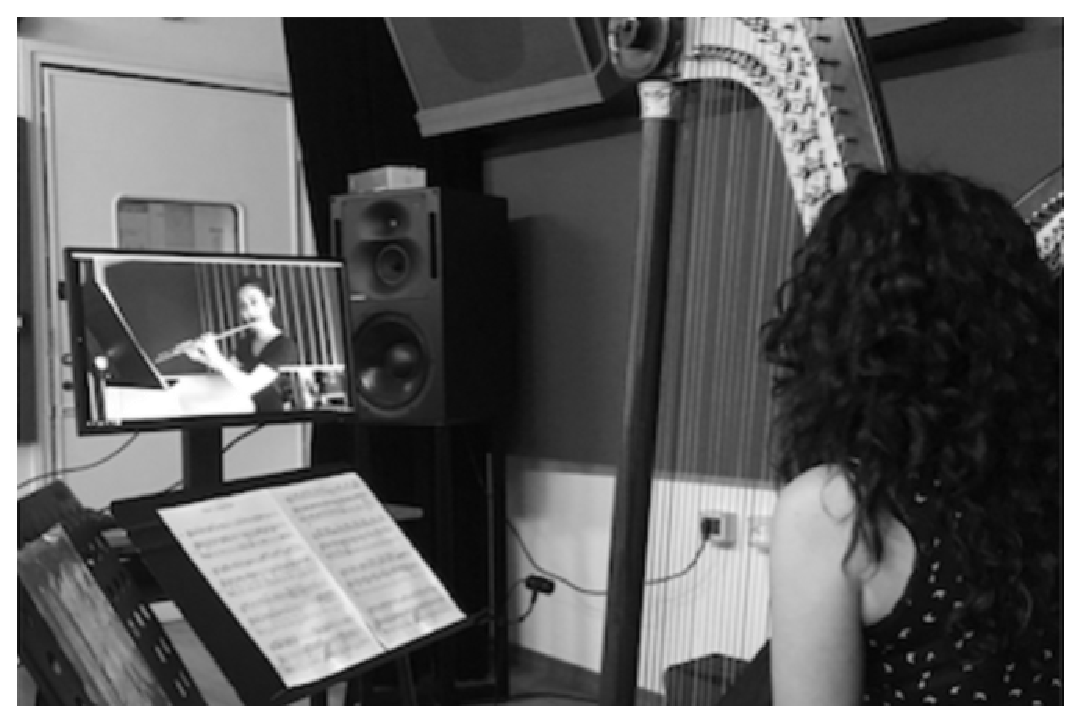
\includegraphics[width=\textwidth]{img/as.eps}
		\caption{View of Room 1}
		\label{subfig:as}
	\end{subfigure}
    \begin{subfigure}[t]{.48\columnwidth}
	\centering        
	%\includegraphics[trim={.5cm 13.7cm 13.5cm .5cm},clip,width=\textwidth]{figures/ann1}
	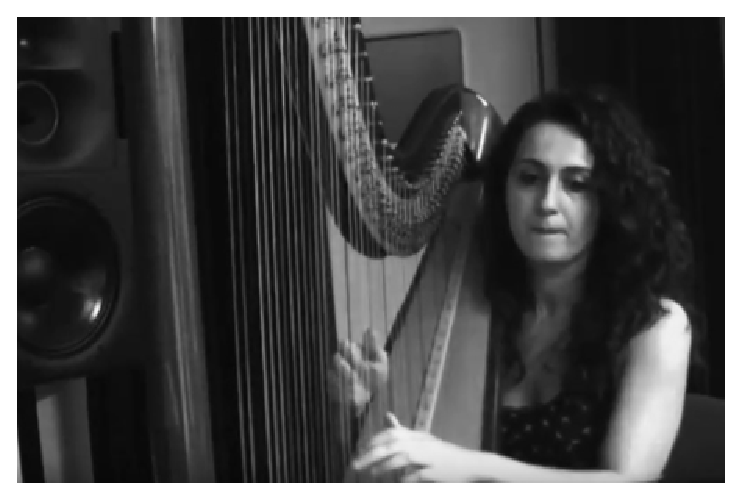
\includegraphics[width=\textwidth]{img/av.eps}
	\caption{View of Musician 1 from Room 2}
	\label{subfig:av}
	\end{subfigure}
    \begin{subfigure}[t]{.48\columnwidth}
	\centering        
	%\includegraphics[trim={.5cm 13.7cm 13.5cm .5cm},clip,width=\textwidth]{figures/ann1}
	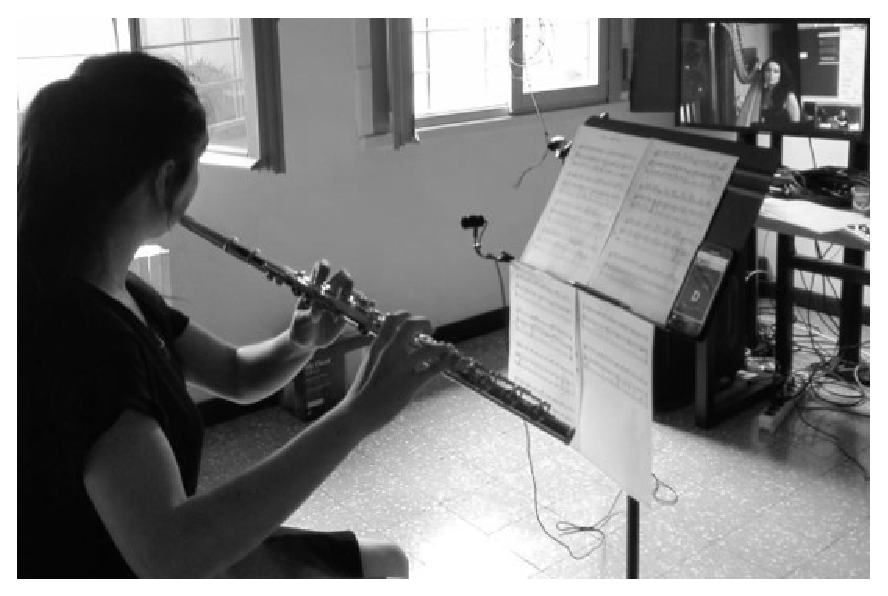
\includegraphics[width=\textwidth]{img/fs.eps}
		\caption{View of Room 2}
	\label{subfig:fs}
	\end{subfigure}
	\begin{subfigure}[t]{.48\columnwidth}
	\centering        
	%\includegraphics[trim={.5cm 13.7cm 13.5cm .5cm},clip,width=\textwidth]{figures/ann1}
	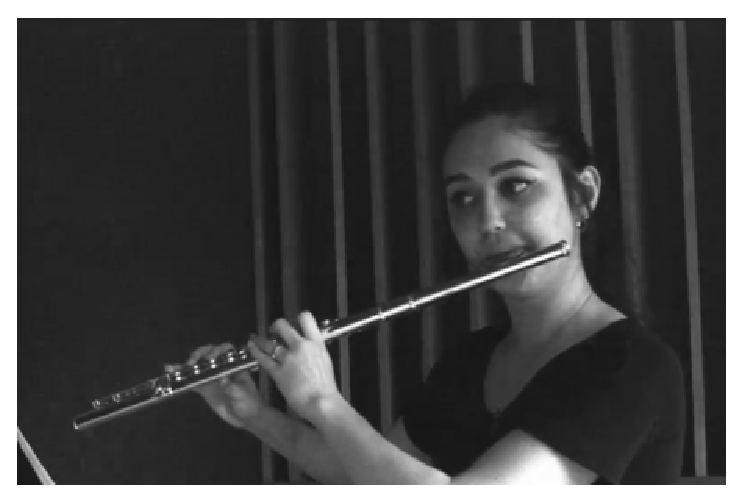
\includegraphics[width=\textwidth]{img/fv.eps}
	\caption{View of Musician 2 from Room 1}
	\label{subfig:fv}
\end{subfigure}

	\quad 
	\caption{View of Rooms 1 and 2 and the corresponding view seen on the screen}\label{fig:afsv}

\end{figure*}

